\documentclass[11pt]{article}
\usepackage{latexsym}
\usepackage{amsmath}
\usepackage{amssymb}
\usepackage{amsthm}
\usepackage{epsfig}
\usepackage[tight]{subfigure}

\usepackage{amsmath}

\DeclareMathOperator*{\minimize}{min}
\DeclareMathOperator*{\maximize}{max}

\DeclareMathOperator*{\argmax}{argmax} % thin space, limits underneath in displays
\DeclareMathOperator*{\argmin}{argmin}

\usepackage{algorithm}
 %on linux you may need to run sudo apt-get install texlive-full to install algorithm.sys
\usepackage{algorithmic}

\usepackage{verbatim}
\usepackage{amsmath,amsfonts,amsthm,bm}


\newcommand{\handout}[5]{
  \noindent
  \begin{center}
  \framebox{
    \vbox{
      \hbox to 5.78in { {#1} \hfill #2 }
      \vspace{4mm}
      \hbox to 5.78in { {\Large \hfill #5  \hfill} }
      \vspace{2mm}
      \hbox to 5.78in { {\em #3 \hfill #4} }
    }
  }
  \end{center}
  \vspace*{4mm}
}

\newcommand{\lecture}[5]{\handout{#1}{#2}{#3}{#4}{#5}}
\newcommand{\collision}[0]{\mathrm{collision}}
\newcommand{\nocollision}[0]{\overline{\collision}}

\newcommand*{\QED}{\hfill\ensuremath{\square}}

\newtheorem{theorem}{Theorem}
\newtheorem{corollary}[theorem]{Corollary}
\newtheorem{lemma}[theorem]{Lemma}
\newtheorem{observation}[theorem]{Observation}
\newtheorem{proposition}[theorem]{Proposition}
\newtheorem{definition}[theorem]{Definition}
\newtheorem{claim}[theorem]{Claim}
\newtheorem{fact}[theorem]{Fact}
\newtheorem{assumption}[theorem]{Assumption}
\newtheorem{note}[theorem]{Note}

% 1-inch margins, from fullpage.sty by H.Partl, Version 2, Dec. 15, 1988.
\topmargin 0pt
\advance \topmargin by -\headheight
\advance \topmargin by -\headsep
\textheight 8.9in
\oddsidemargin 0pt
\evensidemargin \oddsidemargin
\marginparwidth 0.5in
\textwidth 6.5in

\parindent 0in
\parskip 1.5ex
%\renewcommand{\baselinestretch}{1.25}

\newcommand{\btheta}{\boldsymbol{\theta}}
\newcommand{\bz}{\boldsymbol{z}}
\newcommand{\bw}{\boldsymbol{w}}
\newcommand{\bu}{\boldsymbol{u}}
\newcommand{\bv}{\boldsymbol{v}}
\newcommand{\bx}{\boldsymbol{x}}


% \newcommand{\argmin}[1]{\underset{#1}{\operatorname{arg}\,\operatorname{min}}\;}
% \newcommand{\argmax}[1]{\underset{#1}{\operatorname{arg}\,\operatorname{max}}\;}

\begin{document}

\lecture{Statistical Techniques in Robotics (16-831, S22)}{Lecture \#09
  (Wednesday, Febuary 16)}{Lecturer: Kris Kitani}{Scribes: Tzu-Hsuan Yang, Mukun Guo}{Online Gradient Descent \& Norm. Exp. Gradient Descent}

\section{Review}
%This section serves as a review of the previous lecture and any other context required to frame the content of the current lecture. 

%You may format the scribes in any way you like, aside from changing font style, size and page format. Please use subsections and paragraphs to increase the readability of your notes.

%Length requirement 1-2 pages.
Last lecture we studied Online Mirror Descent and Duality, together with some mathematical tools and analysis. We will review some of the core contents.

\subsection{Online Mirror Descent}
Online Mirror Descent provides us a framework that connects many online learning/optimization algorithms. It can be interpreted as a Follow the Regularized leader (FTRL) algorithms with linear loss with convex regularization term, and further gives us a unification of online learning algorithms and more mathematical tools for regret analysis.

In order to establish the connection between OMD and FTRL, we define the following notations.
\begin{enumerate}
    \item $\bz^{(1:t)} = \sum_{i=1}^{t} \bz^{(i)}$  (sum of gradients of linear loss in FTRL-LinLoss)
    \item $\btheta \triangleq -\bz^{(1:t)}$ (parameter of the dual space, sum of gradients in the dual space)
    \item $\btheta^{(t+1)} = \btheta^{(t)} - \bz^{(t)}$ (dual space parameter defined as incremental sum)
    \item $\bw = g(\btheta)$ (mirror/linking function, connect dual space with primal space)
\end{enumerate}

The OMD algorithm is formally written as:
\begin{algorithm}[H]
\caption{Online Mirror Descent (Convex Set $S$, $g: \mathbb{R}^D \rightarrow S$)}
\label{algo:omd}
\begin{algorithmic}[1]
    \FOR{$t=1,2,\;\ldots,\;T$}
        \STATE \textsc{Receive} ($f^{(t)}: W \rightarrow \mathbb{R}$)
        \STATE $\bm\theta^{(t+1)} = \bm\theta^{(t)} - \eta \textbf{z}^{(t)}, \;\;\; \textbf{z} \in \partial f^{(t)}(\textbf{w}^{(t)}) $\hfill $\triangleright$ Dual parameter update 
        \STATE $\textbf{w}^{(t+1)} = g(\bm\theta^{(t+1)})$ \hfill $\triangleright$ Mirror projection, Primal parameter update   
    \ENDFOR
\end{algorithmic}
\end{algorithm}
Note that different choices of regularizer lead to different $g$, and futher result in different algorithms.

\subsection{Duality}
\subsubsection{Convex conjugate}
The motivation for introducing duality is that the dual space provides another way to optimize primal space parameters. Specifically, we can execute optimization in the dual space and mirror in the primal space. The concepts of primal and dual space can be intuitively understood as two ways to parameterize a function:
\begin{enumerate}
    \item \textbf{Primal:} function / value parameterization:
    $\{\psi(w), w\}$
    \item \textbf{Dual:} intercept / slope parameterization: 
    $\{b(\theta), \theta\}$
\end{enumerate}
Assuming we have a smooth convex function, the equation for a convex conjugate is:
\begin{align}
    \psi^*(\theta) = \max\limits_{\textbf{w}} (\langle \theta, w \rangle - \psi(w))
\end{align}
The convex conjugate has some interesting and useful properties:
\begin{enumerate}
    \item The derivative of the conjugate function w.r.t. $\theta$ is the optimal point on the primal function.
        \begin{align}
        \nabla_\theta \psi^*(\theta) = \frac{\partial \psi^*(\theta)}{\partial \theta} = w^*
        \end{align}
    \item The derivative of the primal function is the slope/dual parameter
        \begin{align}
        \nabla_w \psi(w) = \frac{\partial \psi(w)}{\partial w} |_{w=w^*} = \theta
        \end{align}
        Note that Eq.(2) and Eq.(3) together form a nice inverse relationship that links the primal/dual space.
    \item Fenchel-Young Inequality: The complex conjugate computed at $\theta$ is lower bounded by the line equation that is parameterized by $\theta$
        \begin{align}
        \psi^* (\theta) \geq (\langle w, \theta \rangle - \psi(w))
        \end{align}
\end{enumerate}

\subsubsection{Bregman Divergence}
Bregman Divergence describes the error between a linear approximation and a convex function between two points $u$ and $w$. It is defined as as the difference between the rise of the convex function and the linear approximation function:
\begin{align}
    \psi (w) - \psi (u) = \nabla \psi(u)^T (w-u) + D_{\psi}(w||u) \\ 
    D_{\psi}(w||u) = \psi(w) - \psi(u) - \nabla \psi(u)^T (w-u)
\end{align}

\subsection{OMD Regret Bound}
With the above definition and mathematical tools, we can derive the regret bound for Online Gradient Descent.
\begin{align}
    R(\textbf{u}) &\leq \psi(\textbf{u}) -\psi(\textbf{w}^{(1)}) +\sum_{t=1}^{T} D_{\psi^{*}}(-\textbf{z}^{(1:t)}||-\textbf{z}^{(1:t-1)})
\end{align}
where $\psi$ is the regularization function. Note that this is the general regret bound for any OMD algorithms. With different choices of regularization functions, we will have different algorithms and hence different regret bounds.





\section{Summary}

\subsection{Gradient Descent}
Gradient descent is an standard approach for minimizing  differentiable convex functions. The Gradient Descent algorithm is formally written as Algorithm 2. To understand how the gradient descent works, there are three perspectives to explain the algorithm.

\begin{algorithm}[H]
\caption{Gradient Descent}
\label{algo:gd}
\begin{algorithmic}[1]
\STATE $\textbf{w}^{(0)} \leftarrow 0$ 
\FOR{$t=1,\;\cdots,\;T$}
\STATE \textsc{Compute} ($\nabla{f(w^{(t-1)})}$)
\STATE $w_n^{(t)}= w^{(t-1)}-\eta\nabla{f(w^{(t-1)})}$ 
\ENDFOR
\end{algorithmic}
\end{algorithm}
\subsubsection{Perspective 1 : Geometric}
An intuitive but not rigorous explanation is that moving in the direction opposite of the gradient and finally we will reach the local minima. Given that $f$ is a function of convex hypothesis class $\boldsymbol{w}$ : $f : \mathbb{R} ^{N}\rightarrow \mathbb{R}$ at $\boldsymbol{w}$. The gradient $\nabla{f(\boldsymbol{w})}$ can be denoted as a vector of partial derivatives
\begin{align}
    \nabla f(\boldsymbol{w})=\left\{\frac{\partial f(\boldsymbol{w})}{w_{1}}, \cdots, \frac{\partial f(\boldsymbol{w})}{w_{N}}\right\}
\end{align} If we want to find the \textbf{min} of $f$, move in the opposite direction of the gradient. 

\subsubsection{Perspective 2 : Linear Approximation with regularization}
From the previous geometric point of view, it is hard to come up the update rule. So in this perspective, we want to take gradient descent from the view of linear approximation. When $f$ is convex, we can use first order Taylor series approximation to find the lower bound of $f$ at $u$ as
\begin{align}
f(\boldsymbol{u}) \geq f(\boldsymbol{w})+\langle\boldsymbol{u}-\boldsymbol{w}, \nabla f(\boldsymbol{w})\rangle
\end{align}
If we minimize the approximation directly, as the equation shown below, we will get a solution in at negative infinity. 
\begin{align}
\min_{u}\left\{f(w)+(u-w)^{\top} \nabla f(w)\right\}
\end{align}
Therefore, we can introduce a squared L2 norm constraint 
\begin{align}
    \min _{w}\left\|\boldsymbol{w}-\boldsymbol{w}^{(t)}\right\|_{2}^{2}
\end{align}to express the closeness to $w$ and the final objective function becomes a linear loss with quadratic regularization
\begin{align}
    w^{(t+1)}=\underset{w}{\arg \min } \frac{1}{2}\left\|w-w^{(t)}\right\|^{2}+\eta\left(f\left(w^{(t)}\right)+\left\langle w-w^{(t)}, \nabla f\left(w^{(t)}\right) \right\rangle \right).
\end{align}
To get the optimal $w$, taking the partial derivative of objective function wrt $w$ and set to 0. then we can get the Gradient Descent update rule.  
\begin{align}
\frac{\partial \frac{1}{2}\left\|\mathbf{w}-\mathbf{w}^{(t)}\right\|_{2}^{2}+\eta\left(f\left(\mathbf{w}^{(t)}\right)+\left\langle\left(\mathbf{w}-\mathbf{w}^{(t)}\right), \nabla f\left(\mathbf{w}^{(t)}\right)\right\rangle\right)}{\partial \mathbf{w}}=0 
\end{align}
\begin{align}
\left(\mathbf{w}-\mathbf{w}^{(t)}\right)+\eta\left(0+\nabla f\left(\mathbf{w}^{(t)}\right)=0\right.
\end{align}
\begin{align}
\mathbf{w}^{(t+1)}=\mathbf{w}^{(t)}-\eta \nabla f\left(\mathbf{w}^{(t)}\right)
\end{align}
\subsubsection{Perspective 3 : Isometic Quadratic Approximation}
Similar as previous perspective, with Taylor series approximation, we can then use second order approximation to yield
\begin{align}
    f(\boldsymbol{u}) \approx f(\boldsymbol{w})+(\boldsymbol{u}-\boldsymbol{w})^{\top} \nabla f(\boldsymbol{w})+\frac{1}{2}(\boldsymbol{u}-\boldsymbol{w})^{\top} \nabla^{2} f(\boldsymbol{w})(\boldsymbol{u}-\boldsymbol{w})
\end{align}
Since the $\nabla^{2} f(\boldsymbol{w})$ may be hard to compute, we then use Isometric quadratic approximation(unit scaling in all dimension/directions) to rewrite our approximation as 
\begin{align}
    f(\boldsymbol{u}) \approx f(w)+(u-w)^{\top} \nabla f(w)+\frac{1}{2 \eta}(u-w)^{\top} \mathbf{I}(u-w)
\end{align}
where $\eta$ is a tunable scaling parameter. Then the objective function could be written as 
\begin{align}
    \underset{w}{\arg \min } \frac{1}{2}\|u-w\|^{2}+\eta\left(f(w)+(u-w)^{T} \nabla f(w)\right)
\end{align}
By replacing the $u$ with $w$ and $w$ with $w^{(t)}$ we can then obtain the objective function written as 
\begin{align}
    w^{(t+1)}=\underset{w}{\arg \min } \frac{1}{2}\left\|w-w^{(t)}\right\|^{2}+\eta\left(f\left(w^{(t)}\right)+\left\langle w-w^{(t)}, \nabla f\left(w^{(t)}\right) \right\rangle \right).
\end{align}
which is the same equation shown in perspective 2. Therefore, we will get the gradient descent update rule by doing the same steps in perspective 2. 
\begin{align}
\mathbf{w}^{(t+1)}=\mathbf{w}^{(t)}-\eta \nabla f\left(\mathbf{w}^{(t)}\right)
\end{align}

We have seen this update rule may times such as weighted majority, online perceptron, and FTRL.
In conclusion, this update rule comes from \textbf{a quadratic approximation} of the loss function $f$
\subsection{Stochastic Gradient Descent}
Sometimes, the update rule in the gradient descent is expensive to compute because you have to run through ALL the samples in your data set to do a single update for a parameter in a particular iteration. Therefore, to speed up computation, we can use stochastic gradient descent.The algorithm of stochastic gradient descent is formally written as:  
\begin{algorithm}[H]
\caption{Stochastic Gradient Descent}
\label{algo:sgd}
\begin{algorithmic}[1]
\STATE $\textbf{w}^{(0)} \leftarrow 0$ 
\STATE $\eta > 0$ 
\FOR{$t=1,\;\cdots,\;T$}
\STATE $z \sim D$ \hfill $\triangleright$ sample from the data distribution(single sample or mini-batch)
\STATE $v^{(t)}= \nabla{f_z(w^{(t-1)})}$\hfill $\triangleright$ fast to compute(expectation is the true gradient)
\STATE $w^{(t)}= w^{(t-1)}-\eta v^{(t)}$ 
\ENDFOR
\end{algorithmic}
\end{algorithm}
We can observe from the algorithm that instead of running through all the samples points, stochastic gradient sampled a single or mini-bathed from the data(line 4) to calculate the gradient. By doing so, this random approximation of the data set removes the computational burden associated with gradient descent while achieving iteration faster and at a lower convergence rate.
\subsection{Online (Projected Sub-) Gradient Descent (OGD) as Online Mirror Descent (OMD)}
In the lecture, we learned that OGD is OMD with a linear loss and quadratic regularization. To proof this, we start with defining the regularization function as 
\begin{align}
    \psi(\boldsymbol{w})=\frac{1}{2 \eta}\|\boldsymbol{w}\|_{2}^{2}
\end{align}
and the loss function as 
\begin{align}
    f(\boldsymbol{w})=\langle\boldsymbol{w}, \boldsymbol{\theta}\rangle
\end{align}
Then the prediction rule derives from the mirror function becomes  
\begin{align}
    w =\underset{\boldsymbol{w}}{\arg \min }\left\langle\boldsymbol{w},-\boldsymbol{\theta}^{(t+1)}\right\rangle+\frac{1}{2 \eta}\|\boldsymbol{w}\|_{2}^{2}
\end{align}
and $\frac{1}{2 \eta}\|\boldsymbol{w}\|_{2}^{2}$ can be written as $\frac{1}{2 \eta} \sum_{n} w_{n}^{2}$ So, let $\mathcal{L}=\langle w,-\theta\rangle+\frac{1}{2 \eta} \sum_{n} w_{n}^{2}$, we can obtain the optimal parameter by calculating the gradient. 
\begin{align}
    \frac{\partial \mathcal{L}}{\partial w_{n}}=-\theta_{n}+\frac{1}{2 \eta} 2 w_{n}=0
\end{align}
\begin{align}
    w_{n}=\eta \theta_{n}    
\end{align}
which is a projection of the parameter in the dual space to a parameter in the primal space. Hence this is a mirror function and we can define the mirror function for OGD as 
\begin{align}
    g(\theta) = \eta\theta
\end{align}
There are two versions of OGD mirror function. One of them assumes constrained range of sub-gradients with no projection to the weight update rule called online sub-gradient descent, whose algorithm can be found in Algorithm 4. The other one updates the weight with some explicit condition on the feasibility set via projection called online project sub-gradient descent. As shown in Algorithm 5. 
\begin{algorithm}[H]
\caption{Online Sub-Gradient Descent}
\label{algo:osgd}
\begin{algorithmic}[1]
\FOR{$t=1,\;\cdots,\;T$}
\STATE $\boldsymbol{\theta}^{(t+1)}=\boldsymbol{\theta}^{(t)}-\boldsymbol{z}^{(t)}, \quad \boldsymbol{z}^{(t)} \in \partial f^{(t)}\left(\boldsymbol{w}^{(t)}\right)$ \hfill $\triangleright$ Dual parameter update
\STATE $w^{(t+1)}= \eta \boldsymbol{\theta}^{(t+1)}$ \hfill $\triangleright$ Mirror projection
\ENDFOR
\end{algorithmic}
\end{algorithm}
\begin{algorithm}[H]
\caption{Online Proj Sub-Gradient Descent}
\label{algo:osgd}
\begin{algorithmic}[1]
\FOR{$t=1,\;\cdots,\;T$}
\STATE $\boldsymbol{\theta}^{(t+1)}=\boldsymbol{\theta}^{(t)}-\boldsymbol{z}^{(t)}, \quad \boldsymbol{z}^{(t)} \in \partial f^{(t)}\left(\boldsymbol{w}^{(t)}\right)$\hfill $\triangleright$ Dual parameter update
\STATE $w^{(t+1)}=\prod_{\theta \rightarrow S} \eta \theta^{(t+1)}$ \hfill $\triangleright$ Mirror projection 
\ENDFOR
\end{algorithmic}
\end{algorithm}
\subsection{Analysis of Online Gradient Descent}
To discuss the regret bound of OGD, we start from recalling the general OMD regret bound 
\begin{align}
    R(\boldsymbol{u}) \leq \psi(\boldsymbol{u})-\psi\left(\boldsymbol{w}^{(1)}\right)+\sum_{t=1}^{T} D_{\psi^{*}}\left(-\boldsymbol{\theta}^{(t + 1)} \|-\boldsymbol{\theta}^{(t)}\right)
\end{align}
With Bregman divergence, the RHS of OMD regret will become
\begin{align}
   \psi(\boldsymbol{u})-\psi\left(\boldsymbol{w}^{(1)}\right)+\sum_{t=1}^{T} \psi^{*}\left(\boldsymbol{\theta}^{(t+1)}\right)-\psi^{*}\left(\boldsymbol{\theta}^{(t)}\right)-\nabla \psi^{*}\left(\boldsymbol{\theta}^{(t)}\right)\left(\boldsymbol{\theta}^{(t+1)}-\boldsymbol{\theta}^{(t)}\right)
\end{align}
For the L2 norm, the convex conjugate is also L2 norm, then we can rewritten equation 28 as 
\begin{align}
    \frac{1}{2 \eta}\|u\|_{2}^{2}-\frac{1}{2 \eta}\left\|w^{(1)}\right\|_{2}^{2}+\sum_{t=1}^{T} \frac{1}{2 \eta}\left\|\theta^{(t+1)}\right\|_{2}^{2}-\frac{1}{2 \eta}\left\|\theta^{(t)}\right\|_{2}^{2}-\nabla \frac{1}{2 \eta}\left\|\theta^{(t)}\right\|_{2}^{2}\left(\theta^{(t+1)}-\theta^{(t)}\right)
\end{align}
since we know that $\theta^{(t+1)} - \theta^{(t)}$ is constant, we can then compute the gradient to get 
\begin{align}
    \frac{1}{2 \eta}\|u\|_{2}^{2}-\frac{1}{2 \eta}\left\|w^{(1)}\right\|_{2}^{2}+\sum_{t=1}^{T} \frac{1}{2 \eta}\left\|\theta^{(t+1)}\right\|_{2}^{2}-\frac{1}{2 \eta}\left\|\theta^{(t)}\right\|_{2}^{2}-\frac{1}{ \eta}\theta^{(t)}\left(\theta^{(t+1)}-\theta^{(t)}\right)
\end{align}
by rearranging the summation term and plug in definition of dual parameter(equation 32 $\rightarrow$ equation 33) and removing the always positive term(equation 33 $\rightarrow$ equation 34) , we can get 
\begin{align}
    \frac{1}{2 \eta}\|u\|_{2}^{2}-\frac{1}{2 \eta}\left\|w^{(1)}\right\|_{2}^{2}+\sum_{t=1}^{T} \frac{1}{2 \eta}\left\|\theta^{(t+1)} - \theta^{(t)}\right\|_{2}^{2} \\ 
 = \frac{1}{2 \eta}\|\boldsymbol{u}\|_{2}^{2}-\frac{1}{2 \eta}\left\|\boldsymbol{w}^{(1)}\right\|_{2}^{2}+\sum_{t=1}^{T} \frac{1}{2 \eta}\left\|\boldsymbol{\theta}^{(t)}-\eta \boldsymbol{z}^{(t)}-\boldsymbol{\theta}^{(t)}\right\|_{2}^{2} \\ 
 =\frac{1}{2 \eta}\|\boldsymbol{u}\|_{2}^{2}-\frac{1}{2 \eta}\left\|\boldsymbol{w}^{(1)}\right\|_{2}^{2}+\sum_{t=1}^{T} \frac{1}{2 \eta}\left\|-\eta \boldsymbol{z}^{(t)}\right\|_{2}^{2} \\ 
 \leq \frac{1}{2 \eta}\|\boldsymbol{u}\|_{2}^{2}+\sum_{t=1}^{T} \frac{\eta}{2}\left\|z^{(t)}\right\|_{2}^{2}
\end{align}
Define $D=\max \|u\|_{2}, \boldsymbol{u} \in S$ and $G=\max \|\boldsymbol{z}\|_{2}, \boldsymbol{z} \in \partial f(\boldsymbol{w})$
\begin{align}
    R_{OGD}(\boldsymbol{u}) & \leq \frac{1}{2 \eta}\|\boldsymbol{u}\|_{2}^{2}+\sum_{t=1}^{T} \frac{\eta}{2}\left\|\boldsymbol{z}^{(t)}\right\|_{2}^{2} \\
& \leq \frac{D^{2}}{2 \eta}+\frac{\eta}{2} T G^{2}
\end{align}
To find optimal step size $\eta$
\begin{align}
    \frac{d}{d \eta}\left\{\frac{1}{2 \eta} D^{2}+\frac{\eta}{2} G^{2} T\right\}=0 \\
    \eta=\frac{D}{G \sqrt{T}}
\end{align}
By Replacing $\eta$ with $\frac{D}{G \sqrt{T}}$, we get the \textbf{Regret Bound of Online Gradient Descent}
\begin{align}
    R_{O G D} \leq D G \sqrt{T}
\end{align}

\subsection{Online Normalized Exponentiated Gradient Descent}
The algorithm for \textbf{Online Normalized Exponentiated Gradient Descent} (ONEGD) is defined as:
\begin{algorithm}[H]
\caption{Norm-Exponentiated-Gradient ($\eta$)}
\label{algo:onegd}
\begin{algorithmic}[1]
\FOR{$t=1,\;\cdots,\;T$}
\STATE $\bz \in \partial f^{(t)}(\bw^{(t)})$ \hfill $\triangleright$ Dual parameter update
\STATE $\bw^{(t+1)} \propto \bw^{(t)} \exp{(\eta \bz^{(t)})}$  \hfill $\triangleright$ Mirror Projection
\ENDFOR
\end{algorithmic}
\end{algorithm}
We will now show how this algorithm can be derived from OMD with a specific regularization term.

Recall that in OMD, different choices of $g$ (i.e. mirror function) lead to different algorithms. If we define the regularization function as negative entropy, that is:
\begin{align}
    \psi(\bm{w}) = \sum_{k=1}^K  w_k \log w_k \;\;\; \bm{w} \in \mathbb{S}^K
\end{align}
where $\mathbb{S}^K$ is the K-simplex constraint (further discussed in Appendix), and keep the loss function linear:
\begin{align}
    f(\bw) = \langle \bw, \btheta \rangle
\end{align}
Then our prediction rule becomes:
\begin{align}
    \bw^{(t+1)} = & \argmin_{\bw} \langle \bw, -\btheta^{(t+1)} \rangle + \psi (\bw)\nonumber \\
    = & \argmin_{\bw \in \mathbb{S}^K} \langle \bw, -\btheta^{(t+1)} \rangle + \sum_{k=1}^{K} \bw_k \log \bw_k
\end{align}
Add the simplex constraint:
\begin{align}
    \bw^{(t+1)} = \argmin_{\bw} \langle \bw, -\btheta^{(t+1)} \rangle + \sum_{k=1}^{K} \bw_k \log \bw_k + \lambda \left( 1- \sum_k \bw_k\right)
\end{align}
If we view $\lambda$ as the Lagrangian multiplier, then we can define the objective function as:
\begin{align}
    \mathcal{L} = \langle \bw, -\btheta^{(t+1)} \rangle +  \frac{1}{\eta}\sum_{k=1}^{K} \bw_k \log \bw_k + \lambda \left( 1- \sum_k \bw_k\right)
\end{align}
Now, in order to solve the original optimization problem, we would like to find the minimum of the Lagrangian equation. We will take the partial derivative w.r.t. $w_n$, note that above is only the partial derivative w.r.t one element inside $\bw$:
\begin{align}
    \frac{\partial \mathcal{L}}{\partial w_n} = & -\theta_n + \frac{1}{\eta} (1 + \log w_n) - \lambda 
\end{align}
Set the partial derivative to $0$:
\begin{align}
    0 &= -\theta_n + \frac{1}{\eta} + \frac{1}{\eta}\log w_n - \lambda \nonumber  \\
    \frac{1}{\eta}\log w_n &= \theta_n - \frac{1}{\eta} + \lambda \nonumber\\
    \log w_n &= \eta \theta_n - 1 + \eta \lambda \nonumber\\
             &= \eta \theta_n - (1 - \eta \lambda) \nonumber\\
         w_n &= \exp(\eta \theta_n - (1 - \eta \lambda)) \nonumber\\
             &= \frac{\exp(\eta \theta_n)}{\exp (1 - \eta \lambda)}
\end{align}
where $w_n$ is the minimizer for the objective function, thus the minimizer for linear loss and entropic regularization. From the above equation, since the mirror function enforces the geometry of the problem (e.g. probability simplex) we could derive the mirror function that links dual space with primary space, which is:
\begin{align}
    \label{eq:onegd-mirror}
    g(\btheta) = \frac{\exp (\eta \btheta)}{\sum_{n'} \exp (\eta \theta_{n'})}
\end{align}
And the dual parameter update is the same for all OMD algorithms:
\begin{align}
    \btheta^{(t+1)} = \btheta^{(t)} - \eta \bz^{(t)}, \;\;\; \bz^{(t)} \in \partial f^{(t)}(\bw^{(t)})
\end{align}
Now let's make the mirror projection clearer. From Eq. \ref{eq:onegd-mirror} we have:
\begin{align}
    w_n^{(t+1)} = &  \frac{\exp \left(\eta \theta_n^{(t+1)}\right)}{\sum_{n'} \exp (\eta \theta_{n'}^{(t+1)})} \nonumber \\
    = & \frac{\exp \left(\eta (\theta_n^{(t)} - z_n^{(t)})\right) }{\sum_{k} \exp \left( \eta (\theta_k^{(t)} - z_k^{(t)}) \right)} \nonumber \;\;\; \tag*{(Recall the definition of $\btheta$ as incremental sum)}\\  
    \label{eq:onegd_proj}
    = & \frac{\exp (\eta \theta_n^{(t)}) \exp (-\eta z_n^{(t)})}{\sum_k \exp (\eta \theta_k^{(t)}) \exp (-\eta z_k^{(t)})} \cdot \frac{\sum_j \exp (\eta \theta_j^{(t)})}{\sum_j \exp (\eta \theta_j^{(t)})}
\end{align}
By the definition of the mirror function (Eq. \ref{eq:onegd-mirror}):
\begin{align}
    \label{eq:w_def1}
    w_n^{(t)}=\frac{\exp (\eta \theta_n^{(t)})}{\sum_j \exp (\eta \theta_j^{(t)})} \\
    \label{eq:w_def2}
    \sum_k w_k^{(t)} \exp (-\eta z_k^{(t)}) = \sum_k \frac{\exp (\eta \theta_n^{(t)}) \cdot \exp (-\eta z_k^{(t)})}{\sum_j \exp(\eta \theta_j^{(t)}} 
\end{align}
Plug Eq. \ref{eq:w_def1} and Eq. \ref{eq:w_def2} into Eq. \ref{eq:onegd_proj}, we get:
\begin{align}
     w_n^{(t+1)} = & \frac{w_n^{(t)} \exp (-\eta z_n^{(t)})}{\sum_k w_k^{(t)} \exp (- \eta z_k^{(t)})} \;\;\; \\
    \downarrow \nonumber\\
    w_n^{(t+1)} \propto \; & w_n^{(t)}\exp(-\eta z_n^{(t)})
\end{align}
Lastly, it should be easy to see that Hedge algorithm (Algorithm \ref{algo:hedge}) is an unnormalized exponentiated gradient descent algorithm since it has a linear loss function and exponential weights update.
\begin{algorithm}[H]
\caption{Hedge Algorithm ($\beta$)}
\label{algo:hedge}
\begin{algorithmic}[1]
\STATE $\textbf{w}^{(1)}$ $\leftarrow \{w_n^{(1)} = 1\}_{n=1}^N$ 
\FOR{$t=1,\;\cdot;T$}
\STATE \textsc{Receive} $(\bm{x}^(t) \in \{-1, 1\})$ \hfill
\STATE $i \sim \textsc{Multinomial}(\bm{w}^{(t)}/\Phi^{(t)})$ \hfill
\STATE $\hat{y} = h_i(\bm{x}^{(t)})$ \hfill $\triangleright$ Expected 0-1 loss is linear
\STATE \textsc{Receive} $y^t \in \{-1, 1\}$ \hfill
\STATE $w_n^{(t+1)} = w_n^{(t)}e^{-\beta (\bm{1}[y^{(t)} \neq h_n(\bm{x}^{(t)})])}$ \hfill $\triangleright$ Exponential update
\ENDFOR
\end{algorithmic}
\end{algorithm}

%\section*{References}
%Include your references here. Please cite any resources you found useful.	
%Populate the refs.bib file or list your references manually. Be consistent in formatting!
\nocite{*}
{
\bibliography{refs}
\bibliographystyle{abbrv}
}

\section{Appendix}
%This section provides any relevant background material that was not covered in the lectures, but was found to be useful for understanding the material. 
%For example, derivations, theory underlying techniques employed, etc. 

%Additionally, this section can summarizes applications or extensions of these techniques found in the literature. 
\subsection{Comparison between OGD and ONEGD}
We will conduct a simple comparison between \textbf{Online Gradient Descent} and \textbf{Online Exponentiated Gradient Descent}. Note that this comparison was shown in Lecture 7, but it is a good thing to refresh our memory here.

\begin{table}[!h]
\begin{tabular}{|l|c|c|}
\hline
             & \textbf{Online Gradient Descent}                                            & \textbf{Online Exponentiated Gradient Descent}                              \\ \hline
Example      & Perceptron                                                                  & Hedge/GWM, Winnow                                                           \\ \hline
Predictor    & \begin{tabular}[c]{@{}c@{}}linear: \\ \\ $\bw \cdot \bx^{(t)}$\end{tabular} & \begin{tabular}[c]{@{}c@{}}linear: \\ \\ $\bw \cdot \bx^{(t)}$\end{tabular} \\ \hline
Regularization &
  \begin{tabular}[c]{@{}c@{}}quadratic regularization:\\ \\ $\frac{1}{\eta} ||\bw||_2^2$\end{tabular} &
  \begin{tabular}[c]{@{}c@{}}entropic regularization:\\ \\ $\frac{1}{\eta}\sum_n w_n \log (w_n)$\end{tabular} \\ \hline
Update &
  \begin{tabular}[c]{@{}c@{}}additive update:\\ \\ $\bw^{(t+1)}=\bw^{(t)}-\eta \nabla l(y^{(t)}, \hat{y}^{(t)})$\end{tabular} &
  \begin{tabular}[c]{@{}c@{}}exponential update:\\ \\ $\bw^{(t+1)}=\bw^{(t)} \exp (-\eta \nabla l(y^{(t)}, \hat{y}^{(t)}))$\end{tabular} \\ \hline
Regret Bound & \begin{tabular}[c]{@{}c@{}}no regret:\\ \\ $BL\sqrt{2T}$\end{tabular}       & \begin{tabular}[c]{@{}c@{}}no regret:\\ \\ $\sqrt{(T/2) \log N}$\end{tabular} \\ \hline
\end{tabular}
\end{table}

Note that though both Gradient Descent and Exponentiated Gradient Descent are no-regret algorithm, Exponentiated Gradient Descent has a better bound theoretically.

\begin{figure}[!h]
    \centering
    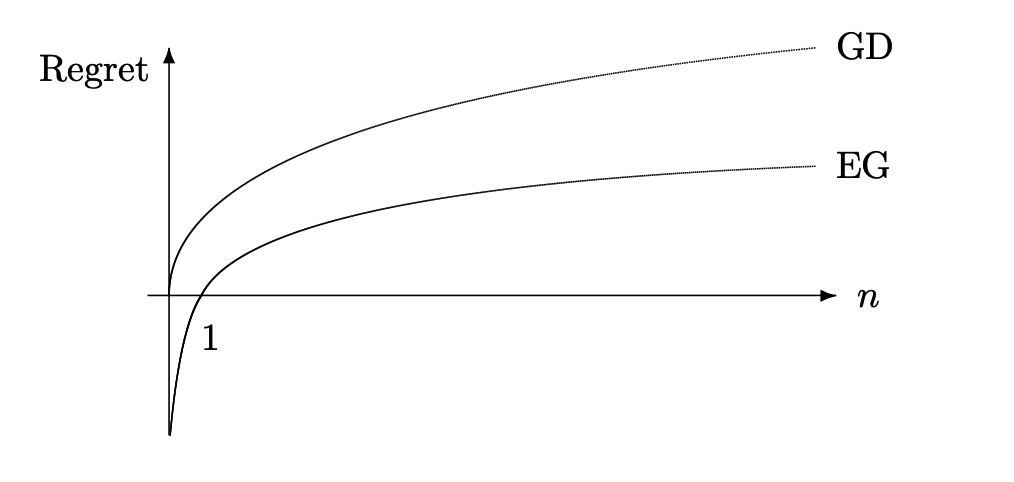
\includegraphics[width=0.7\textwidth]{regret.png}
    \caption{Regret Bound Comparison with $n$ experts}
    \label{fig:comparison}
\end{figure}


\subsection{K-Simplex and Simplex Constraint\cite{enwiki:1072882470}} 
In geometry, a simplex is a generalization of a triangle to arbitrary dimensions. For example,
\begin{enumerate}
    \item 0-simplex is a \textit{point}
    \item 1-simplex is a \textit{line segment}
    \item 2-simplex is a \textit{triangle}
    \item 3-simplex is a \textit{tetrahedron}
\end{enumerate}
Formally, a \textbf{k-simplex} is a defined as:
\begin{align}
    C = \left\{\theta_0 u_0 + \cdots + \theta_k u_k \; \rvert \; \sum_{i=1}^k \theta_i=1 \;\text{and}\; \theta_i \geq 0 \;\text{for}\; i = 0, \cdots, k  \right\}
\end{align}
And the \textbf{probability simplex} or \textbf{standard simplex} is a simplex whose vertices are the $k$ standard unit vectors:
\begin{align}
    \left\{ x \in \mathbb{R}^k: x_0 + \cdots + x_{k-1}=1,x_i\geq 0 \;\text{for}\; i=0,\ldots ,k \right\}
\end{align}

\end{document} % Done!


